\documentclass[a4paper,12pt]{article}
\usepackage[utf8]{inputenc}
\usepackage[T1]{fontenc}
\usepackage[spanish]{babel}
\usepackage{csquotes}
\usepackage{anysize}
\usepackage{graphicx}
\marginsize{25mm}{25mm}{25mm}{25mm}

\title{Contiguity and conditioned reinforcement in probabilistic choice}
\author{Margaret A. McDevitt \and Marcia L. Spetch \and Roger Dunn}
\date{1977}

\begin{document}
{\scshape\bfseries \maketitle}

Se le ha dado poca atención al reforzamiento condicionado. Es tomado solo para representar los efectos del reforzamiento primario demorado. Los procedimientos de reforzamiento probabilístico son de los pocos que permiten separar el reforzamiento primario y el condicionado.

En elección subóptima las palomas muestran preferencia por una alternativa que señala 50\% de reforzamiento mientras sus estímulos correlacionen con la consecuencia final. Cuando los eslabones terminales son largos (30 segundos o más) se maximiza la preferencia subóptima (se llega aproximadamente a indiferencia entre las alternativas).

La contingencia de señalización decrementa la sensibilidad aparente de las palomas a las diferencias entre las tasas de reforzamiento primario de las alternativas ({\itshape creo que nunca había leído esa interpretación}). La elección parece ser determinada principalmente por el reforzamiento condicionado, y los modelos más exitosos se enfocan en él.

Mazur propone que el valor de una alternativa es función de la fuerza de reforzamiento condicionado de sus estímulos, y ésta depende de la demora hasta el reforzamiento primario en su presencia, con lo que el reforzamiento condicionado se vuelve una suerte de puente entre la respuesta y el reforzador primario. Sin embargo, es crítico que para Mazur el valor de la alternativa depende de la fuerza del reforzador condicionado y no de la tasa de reforzamiento condicionado en una alternativa. En procedimientos de reforzamiento probabilístico esto es crítico debido a que, aunque la densidad de reforzamiento de una alternativa disminuya, la demora que anuncian sus estímulos sigue siendo la misma, de modo que se predice que la preferencia se sostenga. Esto coincide con los datos observados. La explicación de Mazur depende de la descripción tradicional de la fuerza de un reforzador condicionada siendo determinada por los parámetros de reforzamientos primario en su presencia. 

Fantino, en cambio, propone que la fuerza de un estímulo como reforzador es una función del grado en que anuncia una mejora en el contexto presente (reducción en demora a reforzamiento primario). Esto sugiere una explicación distinta para la elección subóptima en procedimientos probabilísticos: si todas las elecciones de una alternativa terminan en reforzamiento primario demorado, sus estímulos no proveen de ninguna mejora en el contexto presente, por lo que no funcionan como reforzadores condicionados. Pero si solo la mitad de las elecciones son seguidas de reforzamiento primario demorado, el estímulo asociado con la entrega sí mejora las condiciones actuales (disminuye el tiempo de espera a la comida con relación a la elección actual). Esta diferencia en el valor de los estímulos presentados tras la elección disminuye los efectos de la diferencia en las tasas de reforzamiento primario demorado.

Ambos modelos señalan al reforzamiento condicionado como una variable crítica en el procedimiento.

Este experimento busca medir la eficacia de los estímulos como reforzadores condicionados manipulando su contigüidad con la respuesta de elección a la manera de Belke y Spetch (1994), quienes separaron las respuestas de elección de los estímulos con un {\itshape gap} de 5 segundos en el que las teclas estuvieron oscuras e inoperantes. Se asumió que la presencia de los {\itshape gaps} disminuiría la eficacia de los estímulos como reforzadores condicionados de las respuestas que los produjeron. Belke y Spetch encontraron que la manipulación incrementó la preferencia por la alternativa de 100\% de reforzamiento, lo que indica que la presentación inmediata de los estímulos de eslabones terminales es crítica para la preferencia subóptima. 

La razón entre las tasas de reforzamiento se mantuvo en 2:1 en todas las condiciones. Las condiciones fueron distintas solo en la secuencia de estímulos usados en las demoras. En línea base el estímulo fue presentado de inmediato tras la elección en ambas alternativas.

En Belke y Spetch la presencia del {\itshape gap} incrementó la duración del eslabón terminal en 5 segundos. En este experimento el {\itshape gap} no alteró la duración del eslabón para mantener una demora constante a reforzamiento primario. Además, Belke y Spetch incluyeron {\itshape gap} tras todas las elecciones. En este estudio el {\itshape gap} precede solo a uno, solo a dos, o a todos los estímulos de eslabones terminales. Esto permite investigar el papel de los estímulos en mantener la elección y permite diferenciar mejor los modelos de elección.

Este experimento busca discernir si, como dice Mazur, las alternativas son aproximadamente iguales en fuerza de reforzamiento condicionado, o si la alternativa de 50\% provee mayor reforzamiento condicionado, como dicen Dunn y Spetch. La fuerza relativa de las alternativas se midió comparando la preferencia e línea base con la preferencia en condiciones en las cuales el {\itshape gap} se presentaba solo tras elegir la alternativa de 100\% o solo antecediendo a la omisión de comida en la alternativa de 50\%. Si las alternativas so equivalentes la preferencia debería alejarse de la alternativa con {\itshape gap}, y el desplazamiento debería ser aproximadamente igual sin importar en qué alternativa se coloque el {\itshape gap}. Si la señal de la alternativa de 50\% es más fuerte debería haber un mayor desplazamiento en la preferencia cuando el {\itshape gap} preceda a la señal de comida en la alternativa de 50\% que cuando preceda a la señal de 100\%. 

Mazur propone que la señal de la alternativa de 100\% de reforzamiento funciona como reforzador condicionado, mientras que Dunn y Spetch plantean que podía no adquirir tal valor debido a que no señala una reducción en la demora a la comida más allá de la señalada por la elección. Si funciona como reforzador condicionado imponerle un {\itshape gap} debería desplazar la preferencia hacia la alternativa de 50\% de reforzamiento. Si no, imponerle un {\itshape gap} no debería afectar la preferencia.

Finalmente, para Mazur la señal que anuncia el {\itshape blackout} en la alternativa de 50\% no tiene ningún valor, positivo o negativo. Por otro lado, la formulación de reducción de la demora presume que la presencia de la señal de {\itshape blackout} es necesaria para incrementar el valor de la señal de comida en la alternativa de 50\%, pero esto no especifica cuál debería ser específicamente el valor de la señal de {\itshape blackout}. Una posibilidad es que, como dice Mazur, la señal no tenga valor. Otra es que funcione como castigo condicionado dado que señala un incremento en la demora a la comida. Imponerle un {\itshape gap} no debería tener efecto si la señal no tiene valor, pero debería incrementar la preferencia por la alternativa de 50\% si su valor es negativo.

{\scshape\bfseries Method}

Se usaron cuatro palomas en cajas de condicionamiento con tres teclas, aunque la tecla central no se utilizó. Las teclas se podían iluminar en rojo, blanco, amarillo y verde. 

Se entrenó a las palomas para picar una tecla roja que sería utilizada como eslabón inicial. Después cada ave fue expuesta a seis condiciones en órdenes variables. 

En el eslabón inicial se iluminaban ambas teclas en rojo. Tras una respuesta en cualquiera se apagaban ambos estímulos de eslabón inicial. En algunas condiciones esto iba seguido de un {\itshape gap} de 5 segundos y luego un estímulo de eslabón terminal; en otras se encendía inmediatamente el estímulo. En ambos casos el eslabón terminal terminaba 30 segundos después de la respuesta. En la tecla de 100\% se encendía siempre un mismo color y se entregaban finalmente 3 segundos de acceso a comida. En la tecla de 50\% se podía terminar en 3 segundos de acceso a comida o 3 segundos de {\itshape blackout}. Las consecuencias eran señaladas diferencialmente. No había intervalo entre ensayos ({\itshape ¿por qué no había intervalo entre ensayos?}). Las sesiones duraban 61 ensayos o una hora.

Las condiciones diferían solamente en el {\itshape gap} que precedía a los estímulos del eslabón terminal (figura 1).

\begin{figure}[ht]
        \begin{center}
                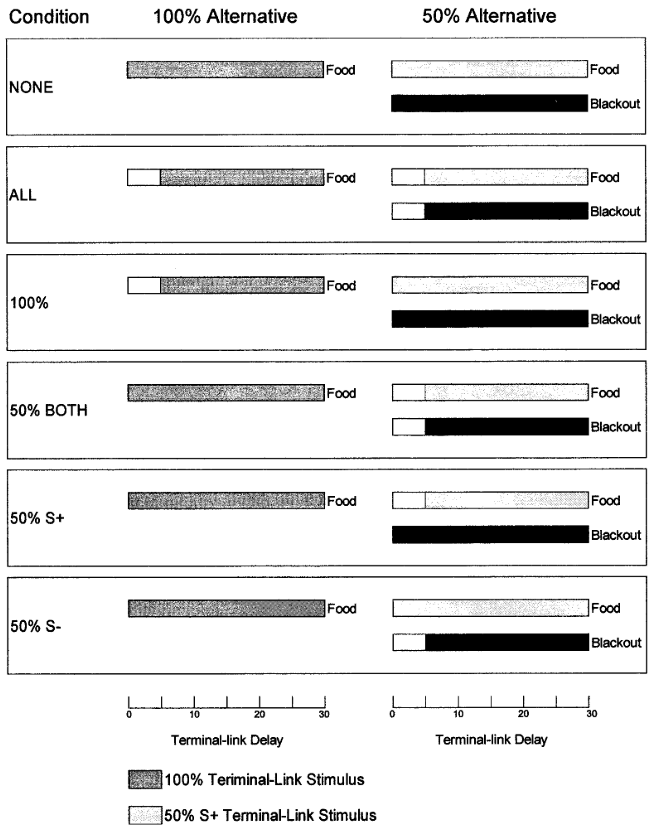
\includegraphics[scale=0.5]{McDevitt1997(1).png}
                \caption{Ubicación de los {\itshape gaps} en cada condición.}
        \end{center}
\end{figure}

Cada ave tuvo un orden y número de sesiones distinto para alcanzar la estabilidad.

Para garantizar el contacto con las contingencias se dieron dos sesiones en un procedimiento de elecciones forzadas al comenzar cada condición.  Además, todas las sesiones comenzaban con ocho ensayos de calentamiento de elección forzada.

Todas las aves tuvieron al menos 15 sesiones por condición, y terminaron cada una hasta cumplir un criterio de estabilidad de nueve sesiones. Los datos reportados son las medias de esas nueve sesiones.

{\scshape\bfseries Results}

Hubo indiferencia entre las alternativas en la condición de línea base (sin {\itshape gaps}). Para todas las aves la elección de la alternativa de 50\% fue mayor en las condiciones de línea base, 100\%, y 50\% S- que en las condiciones en las que el {\itshape gap} precedió al estímulo de 50\% S+. Relativa a la condición de línea base, la preferencia por la alternativa de 50\% fue menos en la condición {\itshape all}, en 50\% {\itshape both} y en 50\% S+. Las preferencias en la condición 100\% u en 50\% S- no fueron distintas de la línea base.

Las tasas de respuesta ante el estímulo positivo fueron mayores en las condiciones 100\% y 50\% {\itshape both} y menores en la condición 50\% S+. Las tasas de respuesta ante el estímulo positivo fueron mayores que ante el estímulo de la alternativa de 100\% en todas las aves en todas las condiciones salvo por 50\% S+. Las tasas de respuesta durante el S- fueron menores excepto en las dos condiciones en las cuales ambas consecuencias de la alternativa de 50\% fueron precedidas por un {\itshape gap} ({\itshape all} y 50\% {\itshape both}).

{\scshape\bfseries Discussion}

Se replica la indiferencia subóptima (preferencia de .55) en la condición {\itshape none} a pesar de la desigualdad entre las tasas de reforzamiento primario de las alternativas. Además se replica la amplia variabilidad individual.

El modelo de {\itshape hyperbolic decay} de Mazur indica que la elección depende solamente del valor condicionado, y que éste se relaciona inversamente a la demora asociada con el reforzador condicionado de cada alternativa. La demora señalada al {\itshape blackout} no se considera reforzador condicionado, por lo que se ignora en el cálculo del valor condicionado. Así, ambas alternativas proveen reforzamiento condicionado y se consideran aproximadamente equivalentes.

La explicación de reducción de la demora indica que la elección depende de reforzamiento primario y condicionado. El primario favorece a la alternativa de 100\%, pero el condicionado favorece a la de 50\%. El reforzamiento condicionado de la alternativa de 50\% es aumentado por la posibilidad de un {\itshape blackout} señalado.

Este experimento probó algunas de las diferencias entre estas explicaciones. Un decremento de las elecciones como función del {\itshape gap} indica el valor del estímulo durante la demora como reforzador condicionado. Variar la posición del {\itshape gap} permitió comparar la fuerza condicionada relativa de intra y entre alternativas.

La comparación de las condiciones {\itshape none} y {\itshape all} permitiría determinar si ambas alternativas proveen el mismo reforzamiento condicionado (Mazur) o la de 50\% provee más (Dunn y Spetch). Todas las aves mostraron mayor preferencia por la alternativa de 50\% en la condición {\itshape none} lo que sugiere que el reforzamiento condicionado era mayor en la alternativa de 50\%. Esto es consistente con el estado especial que se da al S+ en la explicación de reducción de la demora.

Sin embargo, esta reducción en la preferencia por la alternativa de 50\% tampoco es inconsistente con el modelo de Mazur. Según el modelo, la condición {\itshape all} debería debilitar el reforzamiento condicionado más para la alternativa de 50\% que para la de 100\% dado que el {\itshape gap} previo a la presentación de la señal de {\itshape blackout} debe incluirse en el cálculo del valor de la alternativa de 50\%, con lo que se predice un cierto incremento en la preferencia por la alternativa de 100\% en la condición {\itshape all}.

Una mejor comparación está entre las condiciones 100\% y 50\% S+. Dado que en ellas el {\itshape gap} precede a la comida pero en alternativas distintas, de acuerdo con Mazur deberían tener efectos contrarios en la preferencia. Las aves mostraron un mayor cambio en la preferencia en la condición 50\% S+ que en 100\%. Esta comparación da apoyo a la noción de reducción de la demora que indica que la señal que precede comida en la alternativa de 50\% provee más reforzamiento condicionado que la señal de comida de la alternativa de 100\%, y es inconsistente con el supuesto de Mazur de que el reforzamiento condicionado es aproximadamente equivalente entre alternativas.

Hasta ahora solo se ha mostrado que la alternativa de 50\% tiene más reforzamiento condicionado, pero no se ha mostrado si la de 100\% no tiene ninguno. Si ese es el caso, se esperaría que la preferencia fuera igual en las condiciones {\itshape none} y 100\%. En esa comparación los resultados entre sujetos fueron inconsistentes. Una segunda prueba está en la comparación de la condición {\itshape all} y la condición 50\% {\itshape both}. Preferencia por la alternativa de 50\% debería ser mayor en {\itshape all} si imponer un {\itshape gap} en la alternativa de 100\% disminuye su valor, patrón que fue observado en 3 aves. Los resultados no pueden establecer claramente si el estímulo de la alternativa de 100\% es un reforzador condicionado.

Sobre el papel de la señal de {\itshape blackout}, Mazur la ignora y la explicación de reducción de demora sostiene que incrementa el valor de la señal de comida pero no especifica su propio valor. Si es un castigo se esperaría que la preferencia por la alternativa de 50\% fuera menor en la condición 50\% S+ que en 50\% S-. Solo dos aves mostraron ese patrón, y la preferencia general fue mayor en 50\% S+ que en 50\% {\itshape both}. Una segunda comparación pertinente al {\itshape blackout} es {\itshape none} contra 50\% S-: la preferencia por la alternativa de 50\% debería ser mayor en la segunda si la señal de {\itshape blackout} es un castigo condicionado, pero las preferencias no difirieron entre condiciones. Estas comparaciones no dan evidencia suficiente para concluir que la señal del {\itshape blackout} tenga un papel negativo.

Ambas posturas explican la elección subóptima apelando al reforzamiento condicionado, pero difieren en la conceptualización sobre qué determina el valor reforzante. Los resultados de este experimento apoyan a la noción de reducción de la demora que indica que la elección subóptima es influenciada por reforzamiento condicionado que favorece a la alternativa de 50\% y desafían al modelo de {\itshape hyperbolic decay}. Los resultados no permiten concluir que la señal de {\itshape blackout} sea un castigo condicionado, lo que es consistente con la teoría de reducción de la demora. Tampoco se encuentra evidencia que indique que la señal de 100\% de reforzamiento sea un reforzador condicionado, pero la variabilidad entre sujetos nubla toda conclusión.


\end{document}
